\section{Atlas des données}\label{sec:atlas}

Cette section montre la donnée réelle avant toute modélisation. Les figures viennent du notebook \code{v\_demo/CFM\_demo\_features}, exécuté sur Kaggle. Le test n'a pas de labels. Pour le découper par titre, on utilise le titre \emph{prédit} par V3~B (0,635 au LB) : les barres « test » sont donc approximatives, d'autant plus pour les titres que le modèle confond.

\subsection{Une fenêtre, vue de près}
\begin{figure}[H]\centering
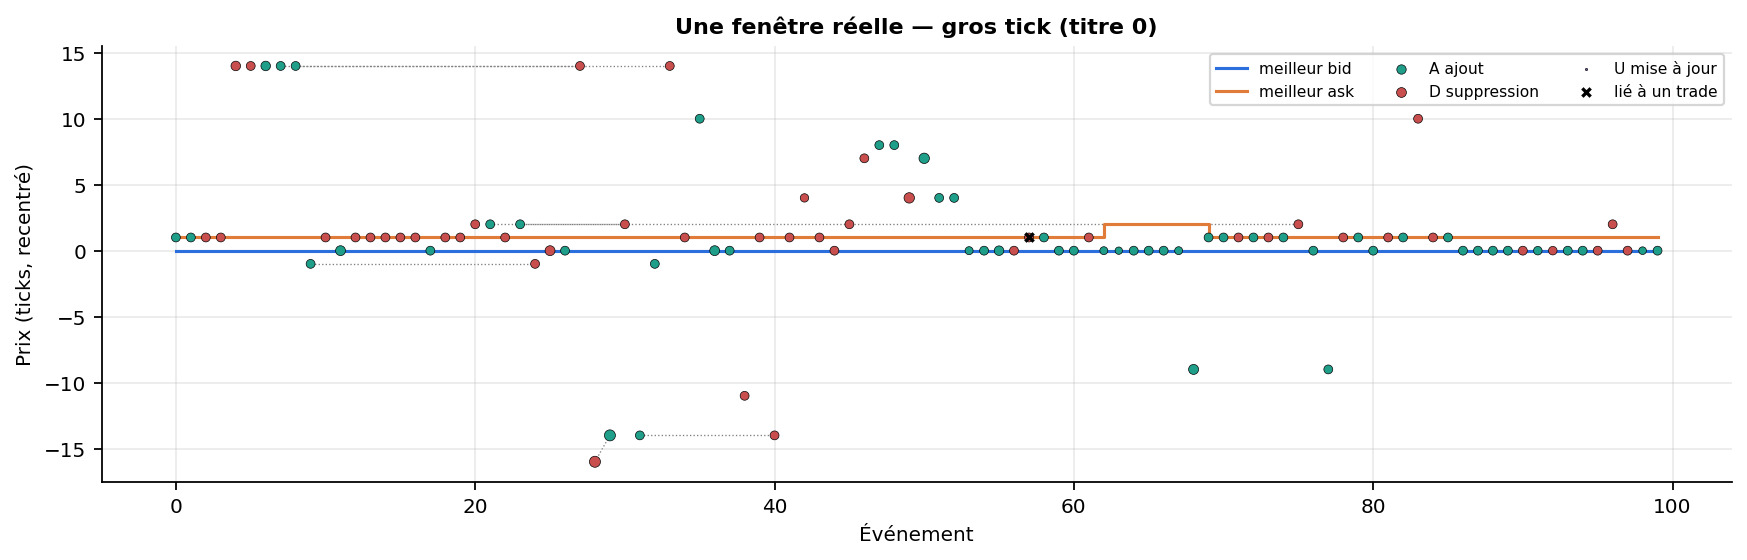
\includegraphics[width=.9\linewidth]{figures/demo_d1_window_big.png}\\[4pt]
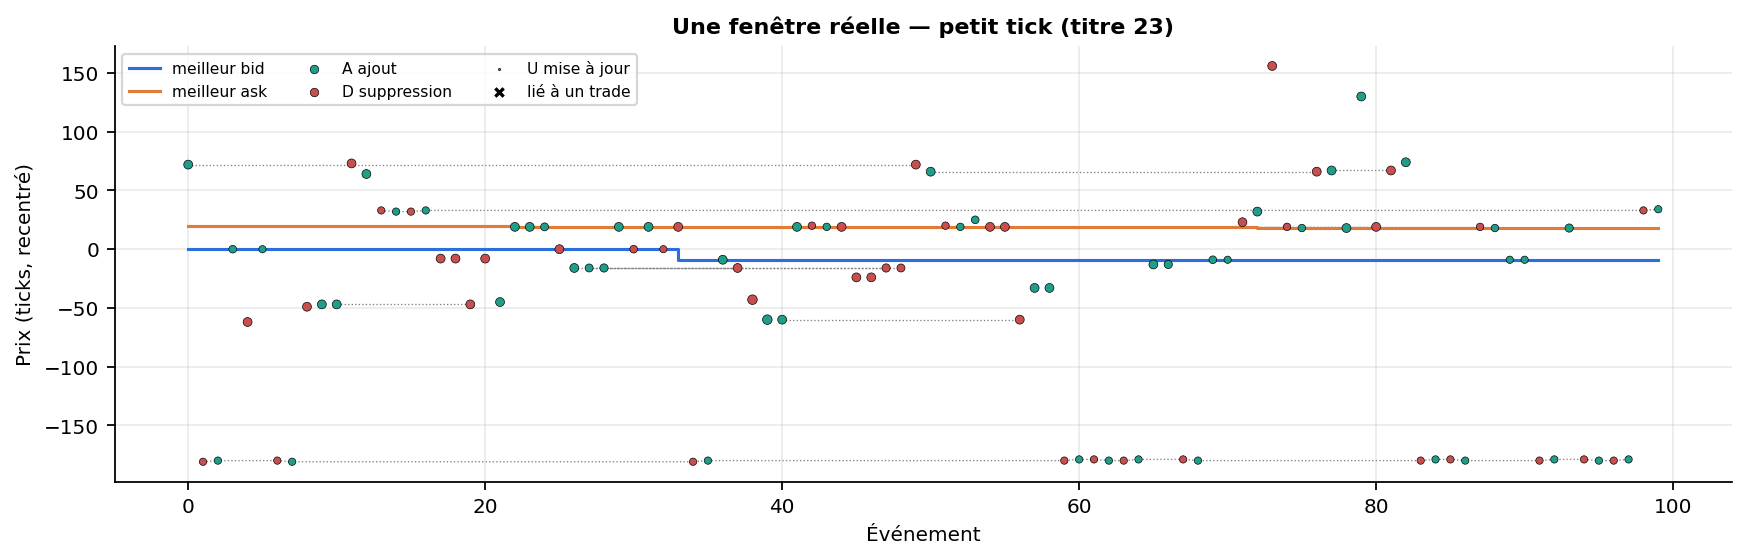
\includegraphics[width=.9\linewidth]{figures/demo_d1_window_small.png}
\caption{Deux vraies fenêtres de 100 événements, prix en ticks recentrés sur le mid initial. En haut, un titre à \emph{gros} tick (titre 0) : le meilleur bid et le meilleur ask sont collés à un tick d'écart et ne bougent presque pas, et les ordres se placent sur quelques niveaux entiers. En bas, un titre à \emph{petit} tick (titre 23) : les ordres s'étalent sur $\pm150$ ticks et le spread vaut plusieurs dizaines de ticks. Exprimées en multiples d'une médiane locale, ces deux fenêtres se ressembleraient bien davantage. C'est l'argument visuel de la section~\ref{sec:unites}.}
\label{fig:atlas-window}\end{figure}

\begin{figure}[H]\centering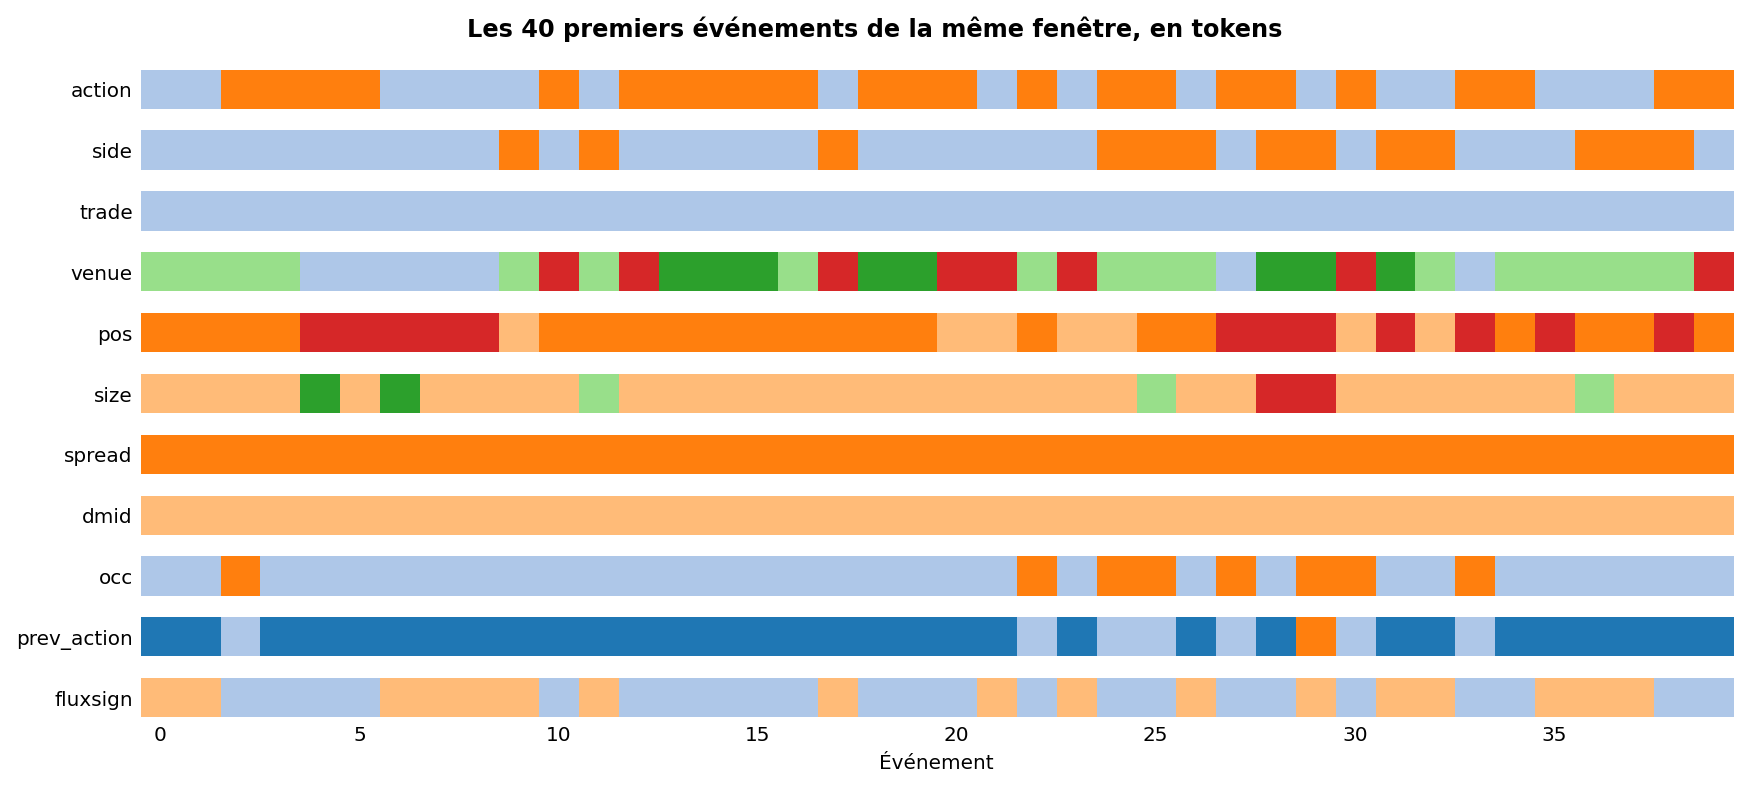
\includegraphics[width=.95\linewidth]{figures/demo_d1_tokens.png}
\caption{Les 40 premiers événements d'une fenêtre, vus par le réseau : une ligne par token (action, côté, trade, venue, position, taille, spread, $\Delta$mid, occurrence, action précédente du même ordre, signe du flux), une couleur par valeur. Certaines lignes sont presque constantes dans une fenêtre (spread, $\Delta$mid) : elles portent le \emph{régime}. D'autres changent à chaque événement (action, venue, occurrence) : elles portent la \emph{dynamique}.}
\end{figure}

\begin{figure}[H]\centering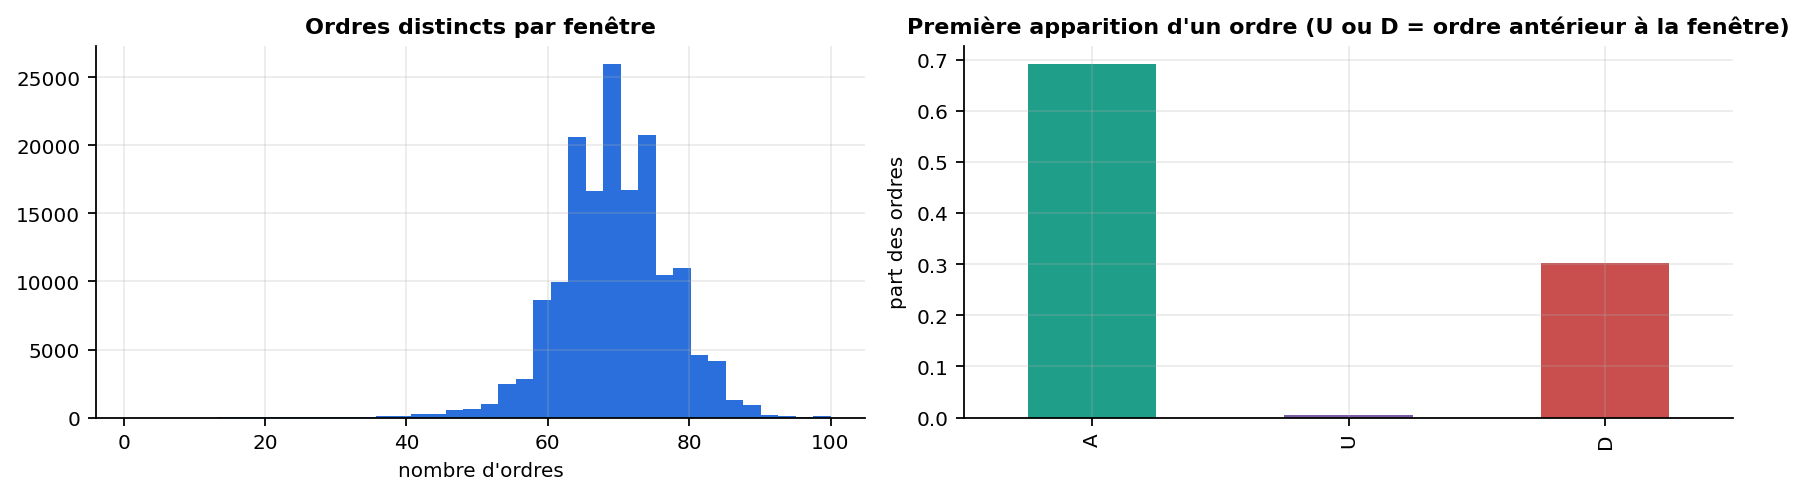
\includegraphics[width=.8\linewidth]{figures/demo_d1_orders.png}
\caption{Ordres par fenêtre. À gauche, une fenêtre de 100 événements touche environ 70 ordres distincts : la plupart n'apparaissent qu'une fois, mais un tiers environ reviennent. À droite, la première apparition d'un ordre est un ajout dans 70\,\% des cas, et une suppression dans 30\,\% : ces ordres ont été placés \emph{avant} la fenêtre. D'où l'intérêt des tokens d'occurrence et d'action précédente du même ordre (section~\ref{sec:ordres}).}
\end{figure}

\subsection{Ce qui distingue les titres}
\begin{figure}[H]\centering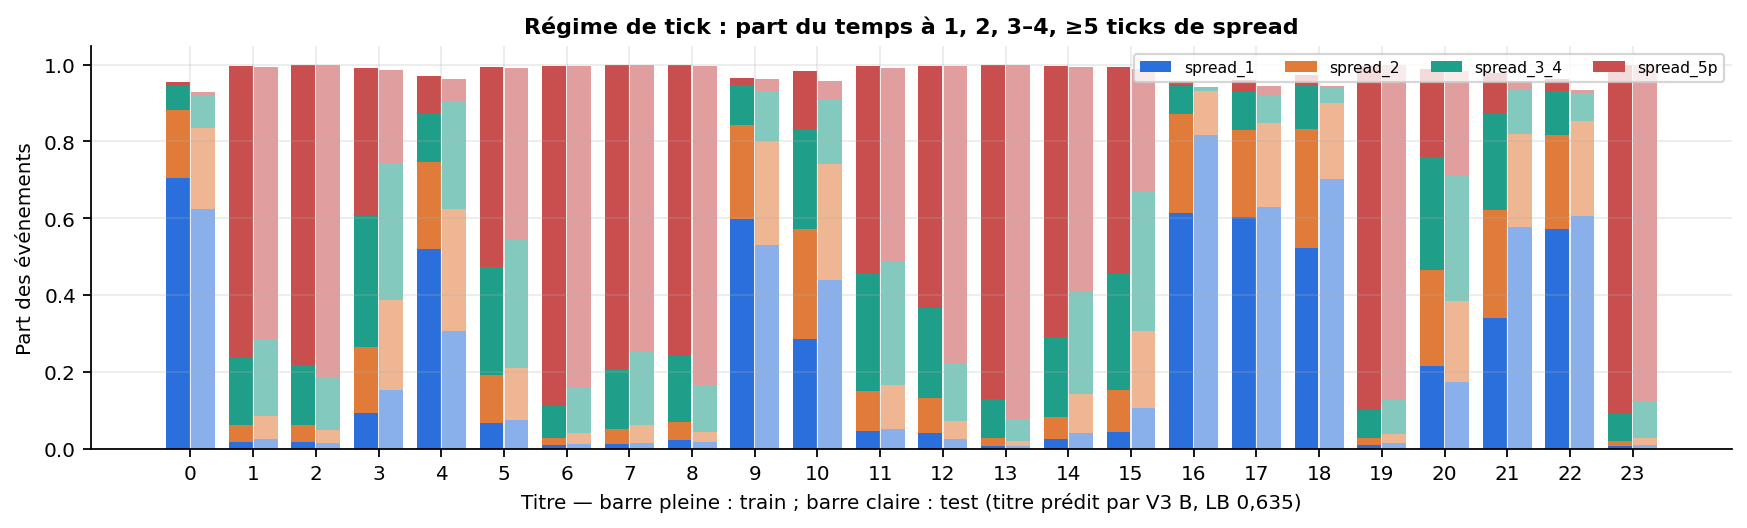
\includegraphics[width=\linewidth]{figures/demo_d2_ticks.png}
\caption{Part du temps passé avec un spread de 1, 2, 3--4 ou au moins 5 ticks, par titre (barre pleine : train ; barre claire : test). Les titres se rangent en deux familles nettes : ceux qui vivent à un tick (0, 9, 16, 17, 22\ldots) et ceux dont le spread dépasse presque toujours 5 ticks. Les barres train et test sont presque identiques : c'est la signature stable par excellence ($\mathrm{KS}\approx0{,}02$, section~\ref{sec:resultats}).}
\label{fig:atlas-ticks}\end{figure}

\begin{figure}[H]\centering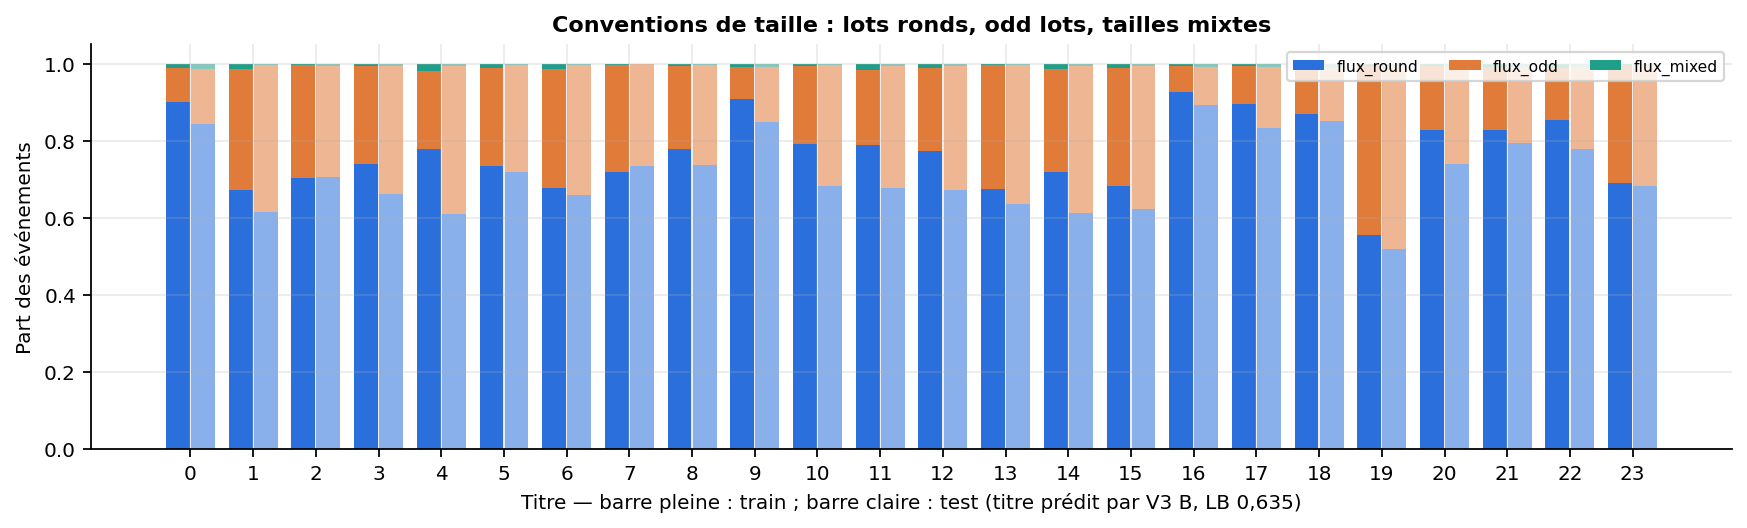
\includegraphics[width=\linewidth]{figures/demo_d2_lots.png}
\caption{Répartition du flux entre lots ronds (multiples de 100), odd lots et tailles mixtes. Les titres se distinguent nettement par leurs conventions de taille. Mais sur la période test, la part d'odd lots augmente pour presque tous les titres. C'est un premier indice de prix plus élevés (section~\ref{sec:aug}).}
\end{figure}

\begin{figure}[H]\centering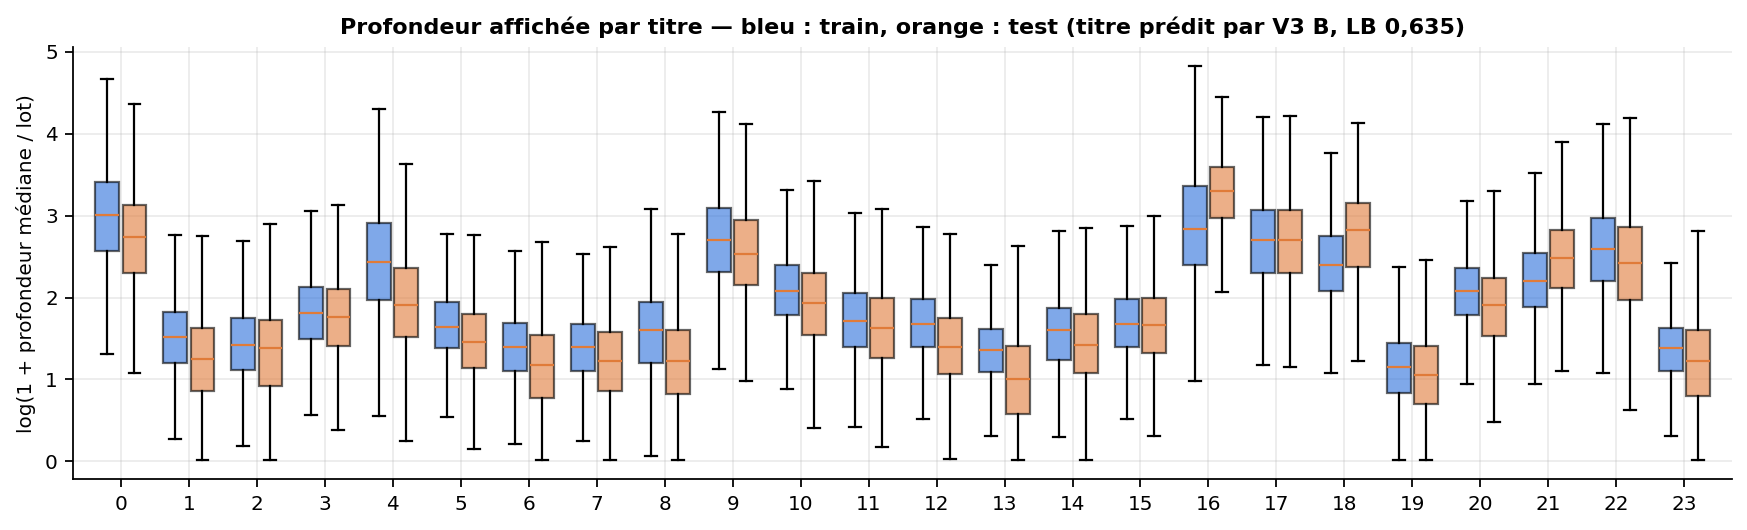
\includegraphics[width=\linewidth]{figures/demo_d2_depth.png}
\caption{Profondeur médiane du carnet (log, en lots) par titre, train en bleu et test en orange. Elle sépare bien les titres, mais elle \emph{baisse} sur le test pour la majorité d'entre eux. C'est le piège de régime de la section~\ref{sec:screening}, et la motivation de l'augmentation et de l'alignement de profondeur.}
\label{fig:atlas-depth}\end{figure}

\begin{figure}[H]\centering
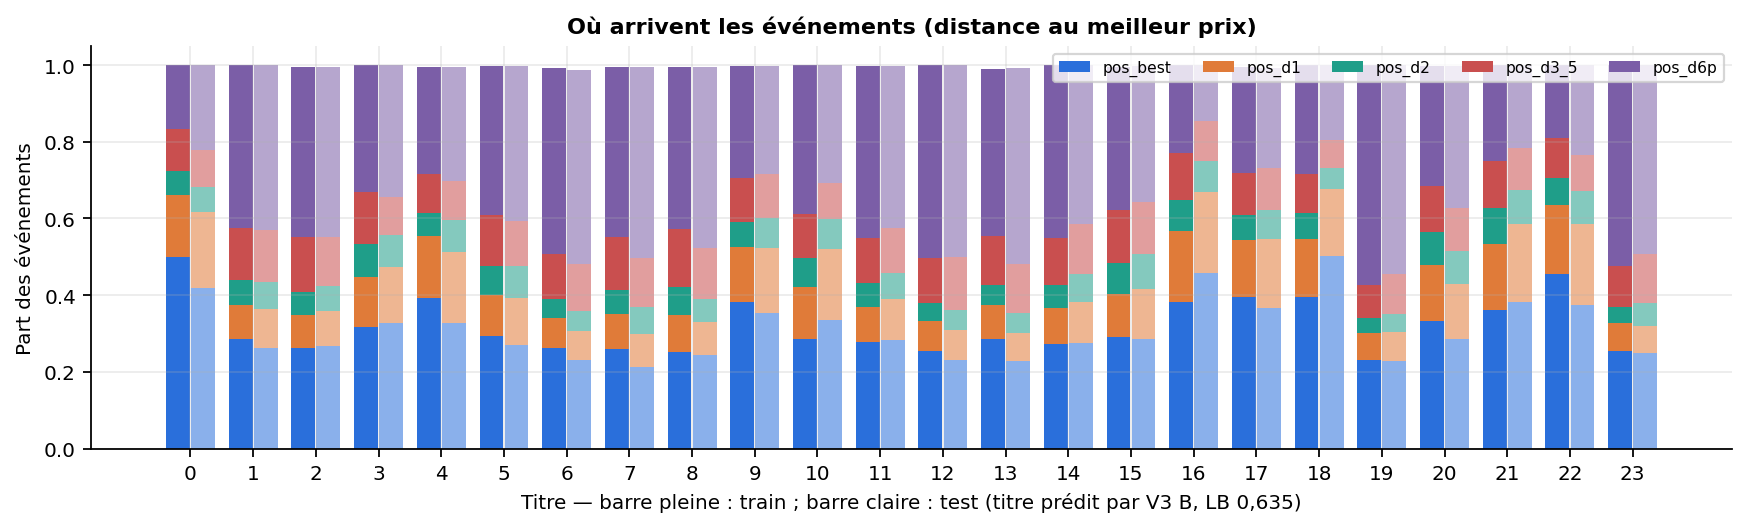
\includegraphics[width=\linewidth]{figures/demo_d2_position.png}\\[4pt]
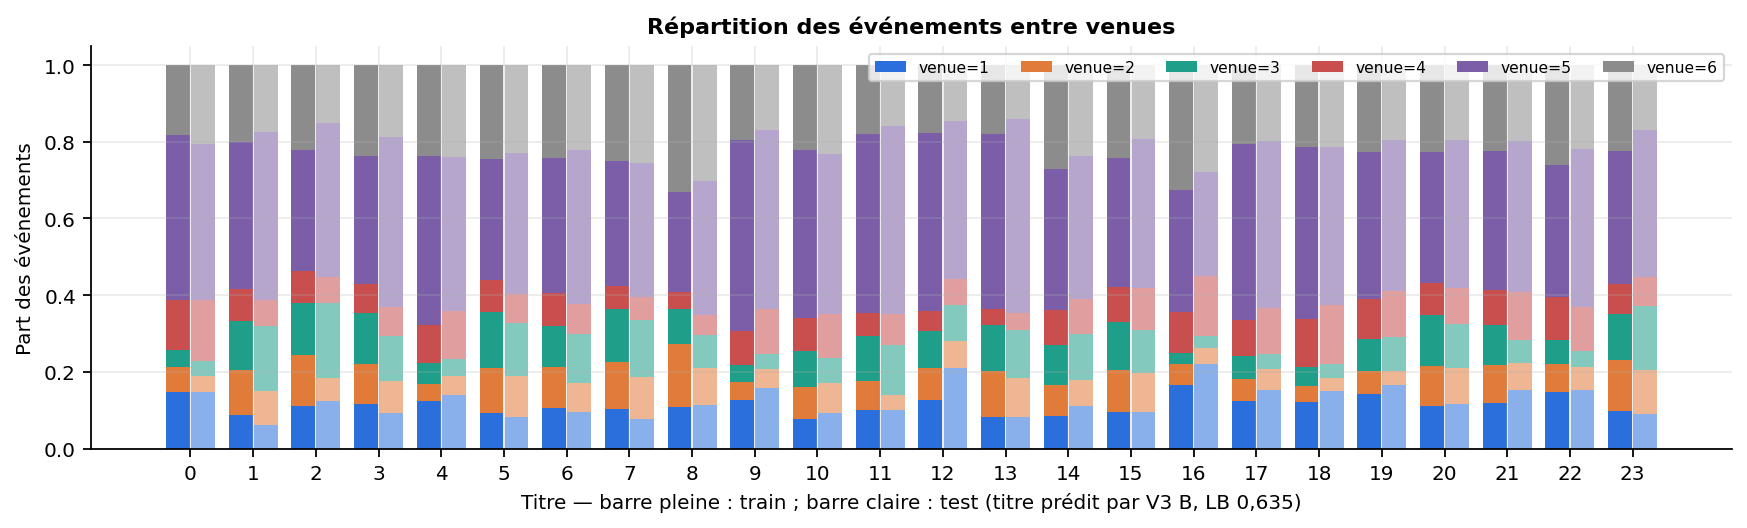
\includegraphics[width=\linewidth]{figures/demo_d2_venues.png}
\caption{En haut, la distance des événements au meilleur prix (au meilleur, à 1, 2, 3--5, 6 ticks et plus). En bas, la répartition entre venues. Les deux varient d'un titre à l'autre et restent stables entre train et test : ce sont des signatures secondaires, mais fiables.}
\end{figure}

\begin{figure}[H]\centering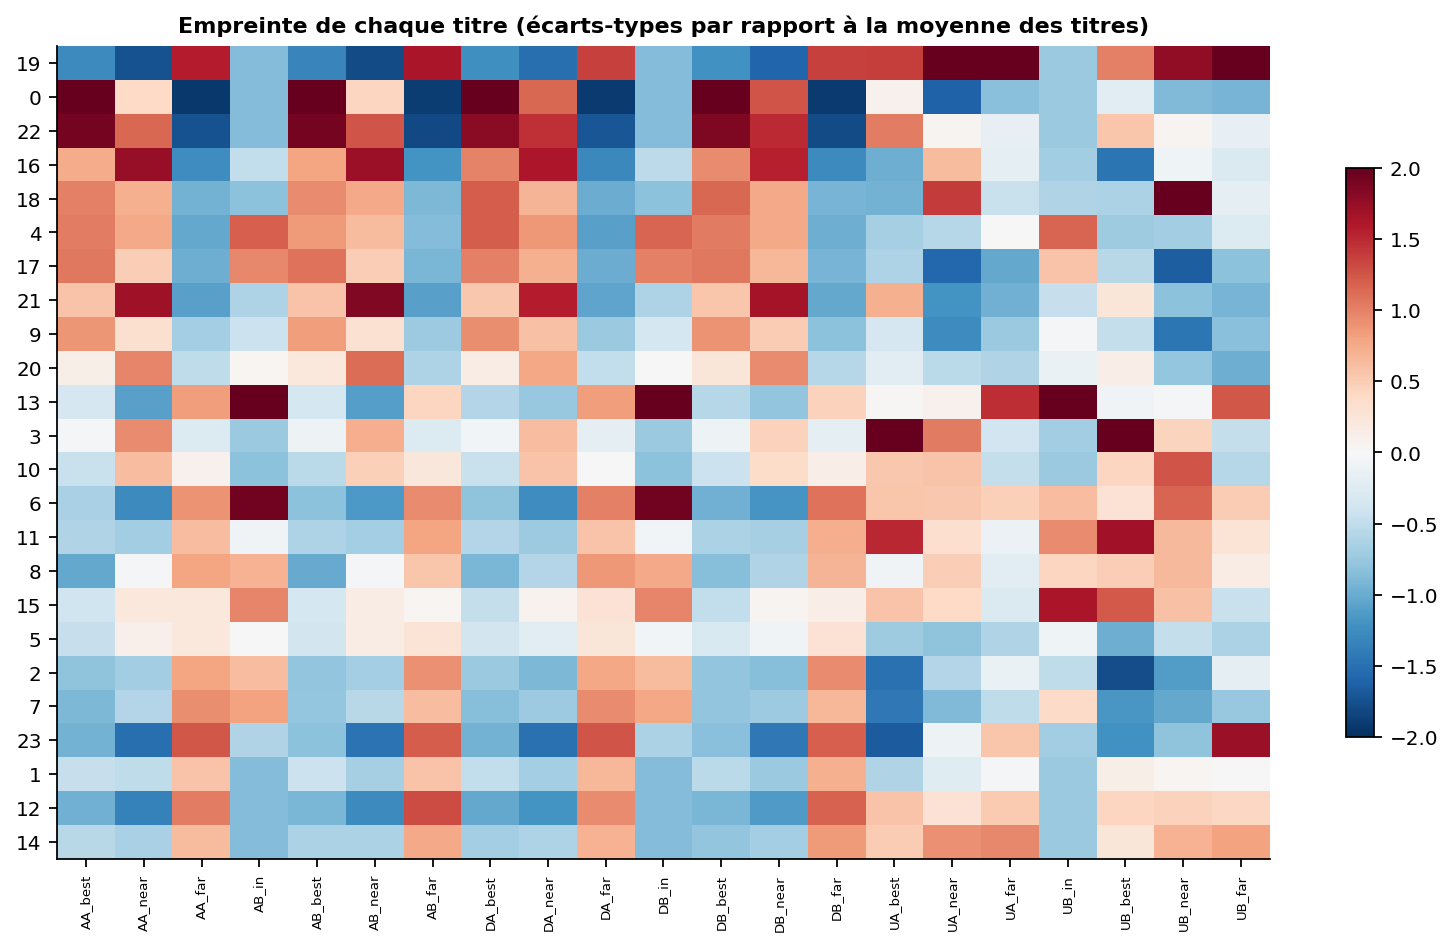
\includegraphics[width=.85\linewidth]{figures/demo_d2_token_fingerprint.png}
\caption{L'empreinte « sac de mots » de chaque titre : fréquence des combinaisons action $\times$ côté $\times$ zone de prix, en écarts-types par rapport à la moyenne des titres. Les titres sont réordonnés par ressemblance. Des blocs de titres aux empreintes voisines apparaissent, par exemple 0 et 22, et ces familles se retrouvent dans les matrices de confusion (figure~\ref{fig:confusion}, famille $\{0,9,17,22\}$).}
\end{figure}

\subsection{Ce qui dérive entre train et test}
\begin{figure}[H]\centering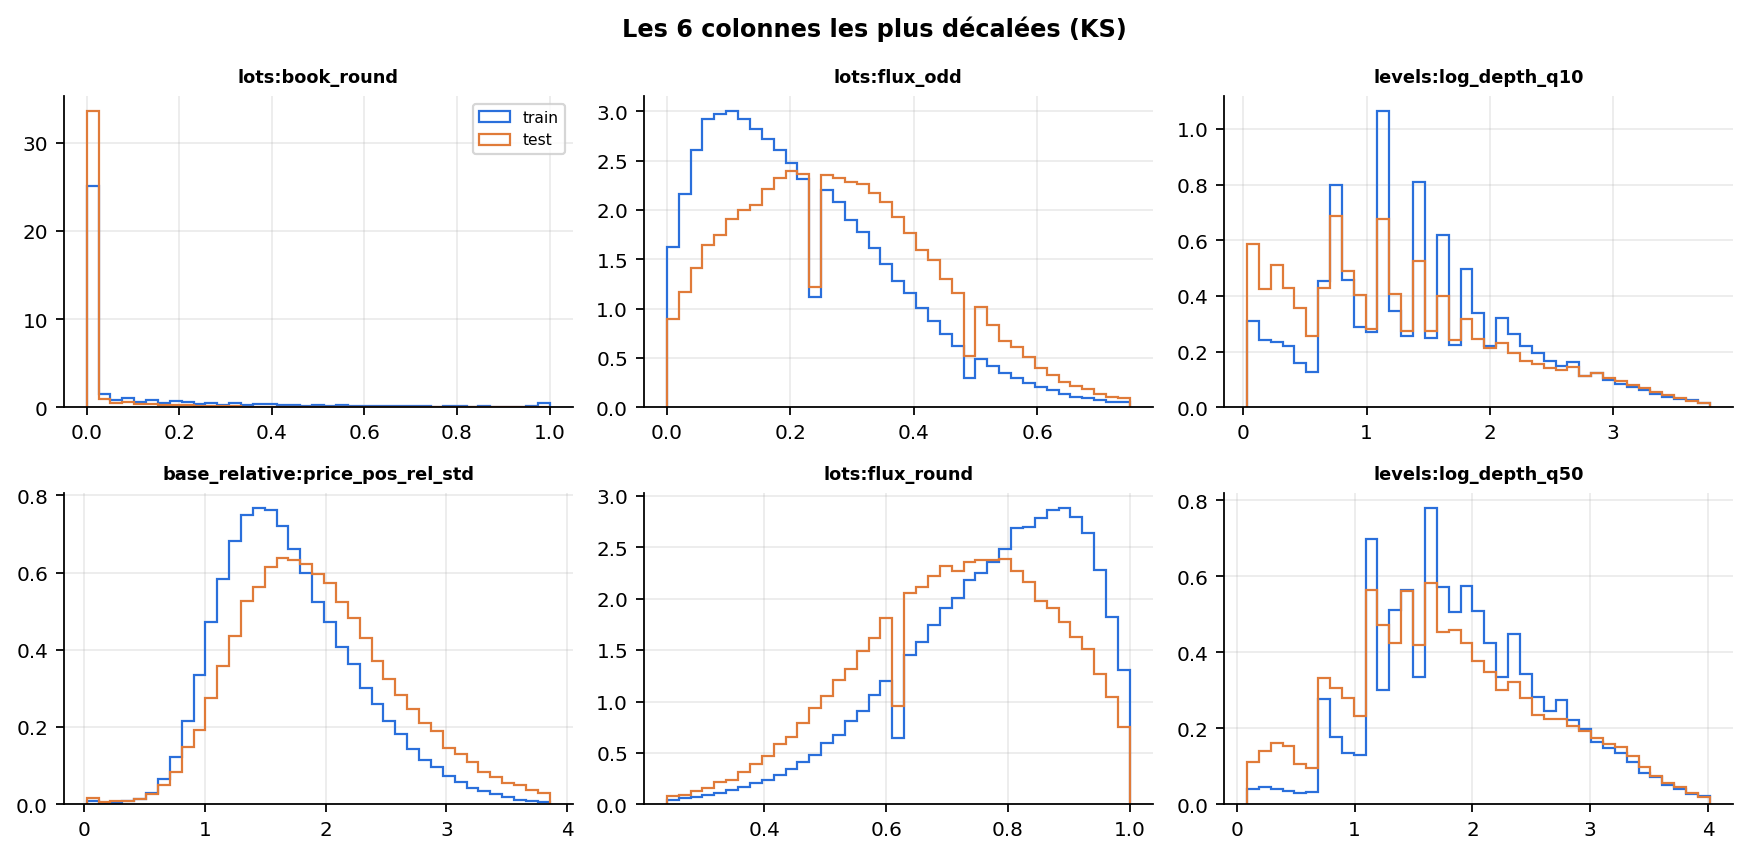
\includegraphics[width=\linewidth]{figures/demo_d3_top_shifts.png}
\caption{Les six colonnes les plus décalées entre train (bleu) et test (orange), au sens du test de Kolmogorov--Smirnov. Toutes appartiennent aux familles \emph{lots} et \emph{profondeur} : moins de lots ronds, plus d'odd lots, des carnets moins profonds. Aucune colonne de tick n'y figure.}
\end{figure}

\begin{figure}[H]\centering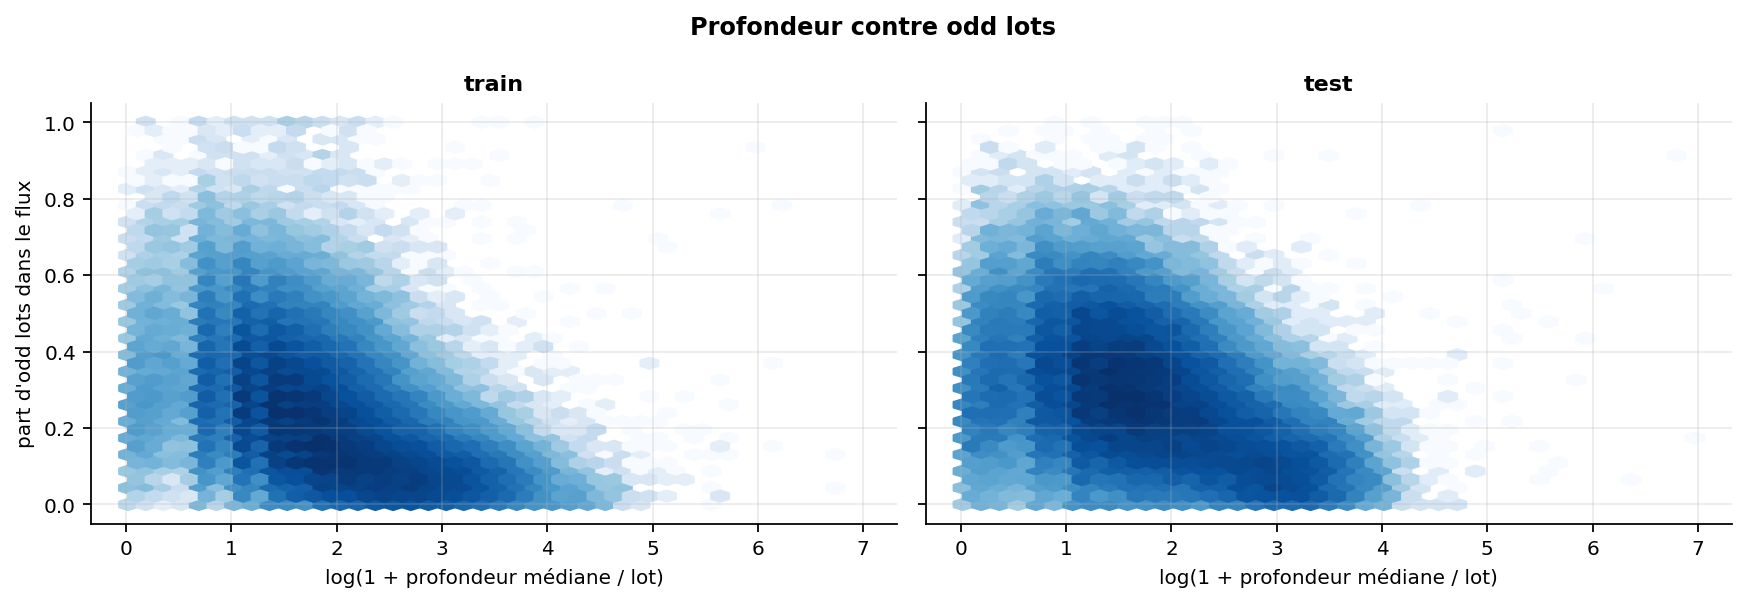
\includegraphics[width=.85\linewidth]{figures/demo_d3_depth_vs_oddlots.png}
\caption{Part d'odd lots en fonction de la profondeur, train contre test. La relation est décroissante dans les deux périodes, et le nuage du test glisse vers les carnets moins profonds et plus riches en odd lots. Un même mécanisme, des prix plus élevés, expliquerait les deux décalages à la fois : à valeur égale, moins d'actions par ordre.}
\end{figure}

\subsection{La vie des ordres}
\begin{figure}[H]\centering
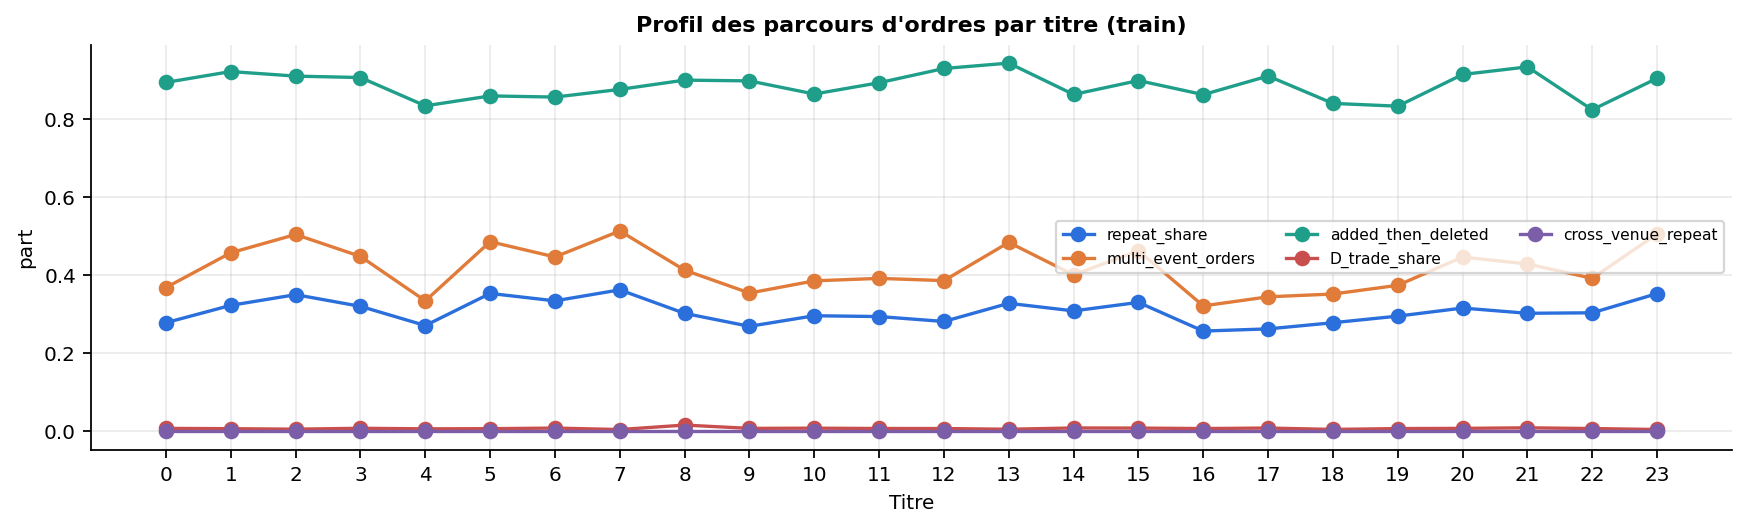
\includegraphics[width=.49\linewidth]{figures/demo_d4_profiles.png}\hfill
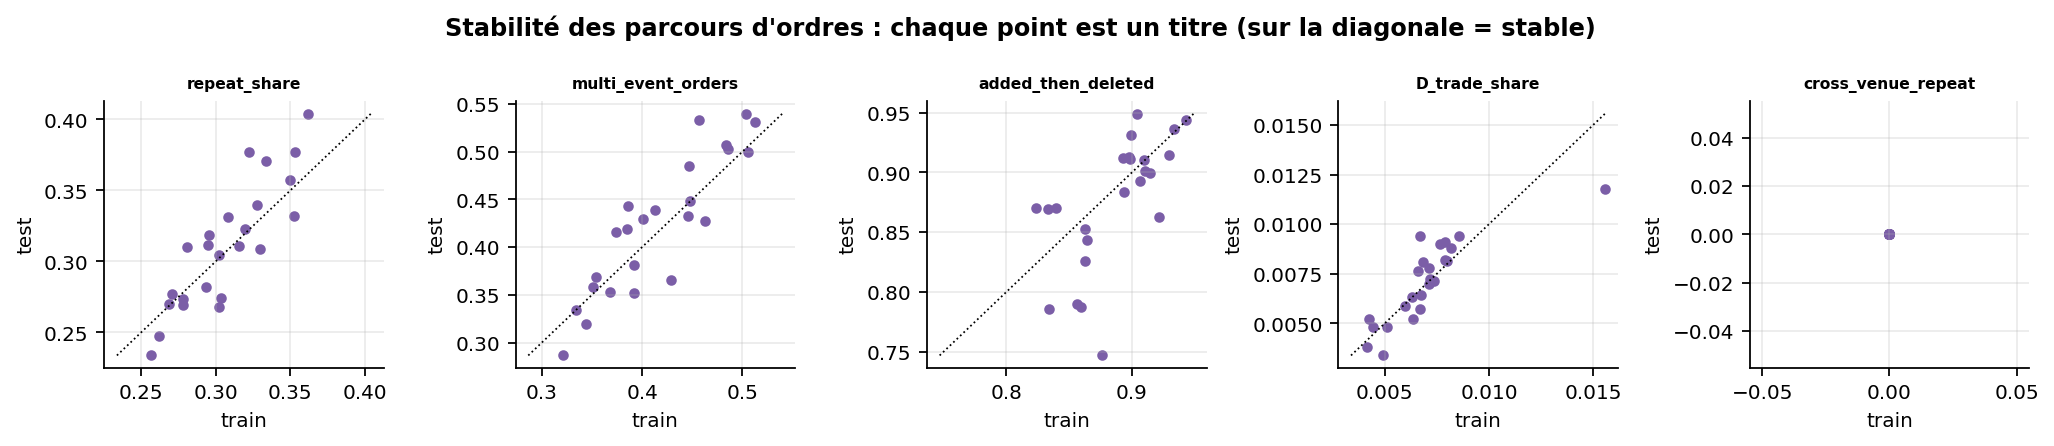
\includegraphics[width=.49\linewidth]{figures/demo_d4_train_vs_test.png}
\caption{À gauche, des profils de parcours d'ordres par titre : part d'ordres ajoutés puis supprimés dans la fenêtre (83 à 94\,\%), part d'ordres à plusieurs événements (33 à 50\,\%), part de répétitions. Les ordres exécutés sont rares. À droite, chaque point est un titre, train en abscisse et test en ordonnée. Les points restent proches de la diagonale : contrairement à la profondeur, la façon dont les ordres vivent et meurent est stable d'une période à l'autre.}
\end{figure}
